\documentclass[tikz]{standalone}
\usepackage{pgfplots}
\pgfplotsset{compat=1.14}
\begin{document}
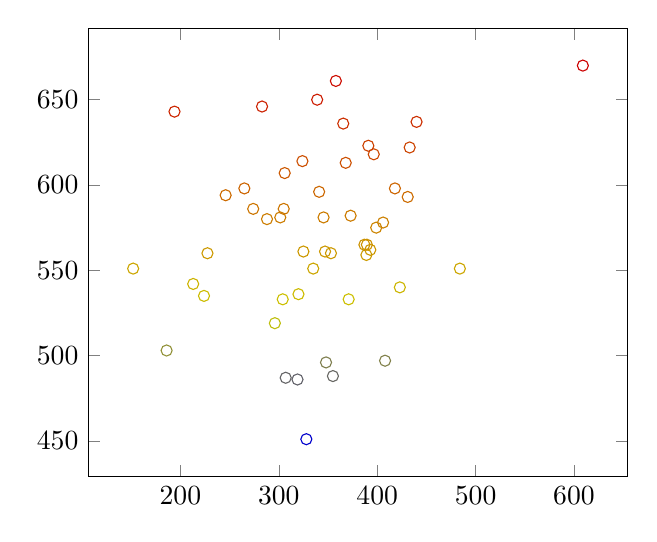
\begin{tikzpicture}
\begin{axis}[]
 \addplot [only marks, mark=o, scatter] coordinates {(609,670) (484,551) (440,637) (433,622) (431,593) (423,540) (418,598) (408,497) (406,578) (399,575) (396.5,618) (393,562) (391,623) (389.5,565) (389,559) (387,565) (373,582) (371,533) (368,613) (365.5,636) (358,661) (355,488) (353,560) (348,496) (347,561) (345.5,581) (341,596) (339,650) (335,551) (328,451) (325,561) (324,614) (320,536) (319,486) (307,487) (306,607) (305,586) (304,533) (301.5,581) (296,519) (288,580) (283,646) (274,586) (265,598) (246,594) (227.5,560) (224,535) (213,542) (194,643) (186,503) (152,551)};
\end{axis}
\end{tikzpicture}
\end{document}